%!TEX root = ../dokumentation.tex

\chapter{Hardware}

Im folgenden Kapitel werden die elektronischen Hardwarekomponenten, sowie deren Verbindungen untereinander vorgestellt. 

Die einzelnen Komponenten lassen sich in drei große Funktionsbereiche klassifizieren.

Der erste Bereich beinhaltet die Distanzbestimmung. Diese wird durch den Lidar-Sensor realisiert.
Der zweite Funktionsbereich ist das Ausrichten des Sensors in zwei Achsen. Beinhaltet sind die zwei Schrittmotoren mit der damit verbundenen Ansteuerung durch Motortreiber. \\
Die automatisierte Kalibrierung stellt den dritten Funktionsbereich dar. Dabei wird über eine Lichtschranke die horizontale Ausrichtung des Sensors bei jedem Start der Anwendung auf eine vordefinierte Ausgangsposition gesetzt. Das Selbe wird durch einen Gyrosensor für die vertikale Ausrichtung ermöglicht.

Als Rechen- und Steuereinheit für das gesamte System wird ein Raspberry Pi verwendet. Dieser bietet sich aufgrund des geringen Preises, der vielen GPIOs und der Unterstützung aller benötigten Datenübertragungsprotokolle an. Zudem reicht die Rechenleistung für das Ansteuern aller Komponenten, sowie das Auswerten und Speichern der Messdaten aus.\\

\section{Funktionseinheit Distanzbestimmung}


\subsection{TF MINi}

Bei der Auswahl des Lidar Sensors spielen Preis, Verfügbarkeit, Messfrequenz, Auflösung, Genauigkeit und messbare Entfernung eine Rolle.


\begin{wrapfigure}{r}{5cm}
	\vspace{-22pt}
	\hspace{5mm}
	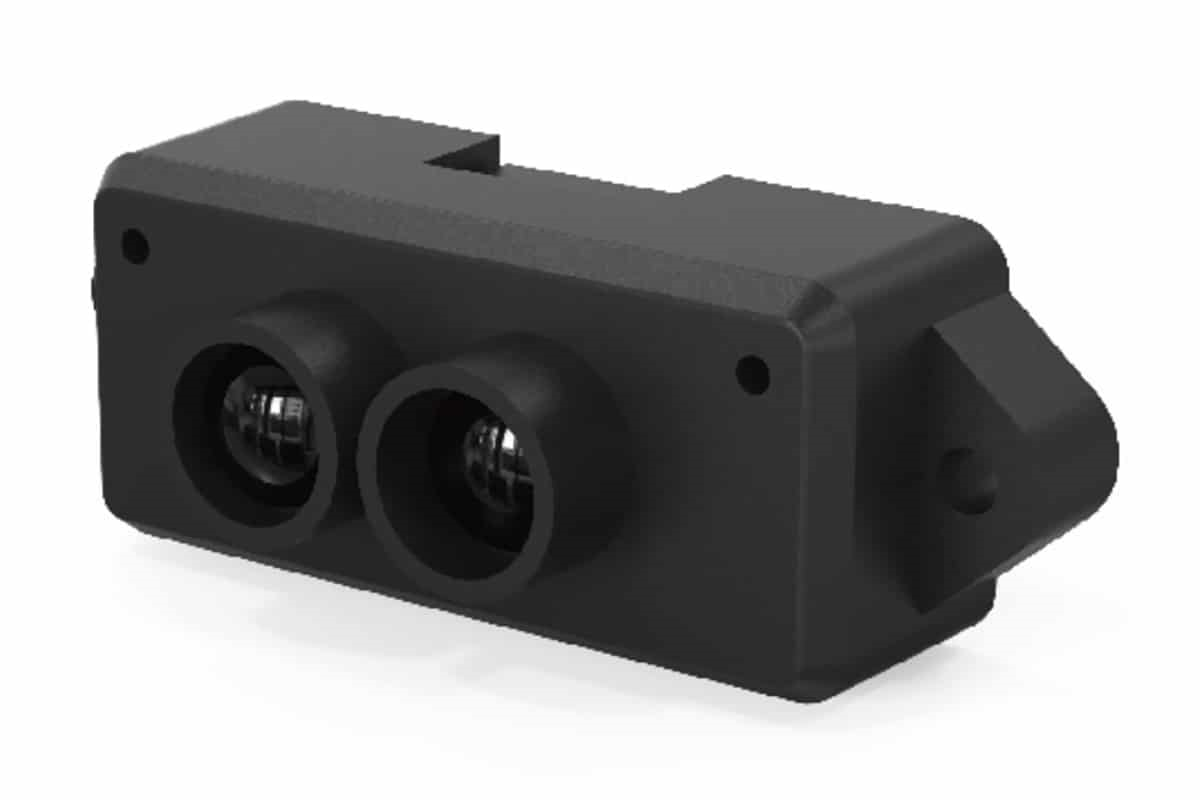
\includegraphics[width=4cm]{images/Hardware/TFmini.png}
	\caption{TFmini}
	\vspace{-10pt}
	
\end{wrapfigure}

Als Sensor wird ein „TF MINI LiDAR“ von dem Hersteller „Seeed Studio“ verwendet. Dieser arbeitet mit auf dem Prinzip der Phasendiffernz wie in Kapitel … beschrieben.\\
Der Arbeitsbereich liegt von 30 cm bis 1200 cm mit einer Auflösung von 1 cm. In dem Messbereich kleiner als 600 cm beträgt die Genauigkeit 1 \%. Zwischen 600 cm und 1200 cm 2 \%. Die Messfrequenz beträgt maximal 100 Hz.\\
Der Sensor arbeitet mit einer Versorgungsspannung von 4.5 V – 6 V bei einem durchschnittlichen Strom von 120 mA. Das Kommunikations-Interface ist UART mit eine Logikspannung von 3.3 V

Die Entscheidung viel auf diesen Sensor, da das Preis-Leistung Verhältnis sehr gut ist. Zudem reicht der messbare Bereich für den zuvor definierten Standardraum. Die Kommunikation über UART ist mit dem Raspberry Pi realisierbar und die 100 Hz reichen für Messungen, die nicht auf Geschwindigkeit ausgelegt sind, aus. Sensoren mit einer deutlich höheren Messfrequenz sind um vielfaches teurer.\\
Zudem ist der Sensor nur 42x15x16 mm groß, wodurch er sehr gut auf der dafür vorgesehenen Aluminiumhalterung montiert werden kann. 


\subsection{VLX...}


\section{Funktionseinheit Ausrichtung des Sensors}

Der Sensor wird durch je einen Schrittmotor in der horizontalen als auch vertikalen Richtung bewegt. Die vertikale Ausrichtung erfolgt dabei direkt. Der Sensor ist über eine Adapterplatte mit der Welle des Schrittmotors verbunden. Dadurch werden Bewegungen des Schrittmotors 1:1 auf den Sensor übertragen.\\
Die horizontale Ausrichtung erfolgt zusätzlich über ein Getriebe mit einem Riemen zur Kraftübertragung. Das Übersetzungsverhältnis entspricht 1:6. 

\subsection{Schrittmotoren}
Das drehen der Basis übernimmt ein bipolarer Hybrid-Schrittmotor der Bauform Nema 17 und einem Vollschrittwinkel von 1.8°. Der Maximalstrom beträgt 1.2 A pro Phase bei einer Spannung von 4V.\\
Dieser Motor wurde gewählt, da er genug Drehmoment aufbringt, um die gesamte Basis drehen zu können. Das hohe Haltemoment verhindert ungewolltes Verdrehen der Basis während der Messung. Dadurch ist das System fehlerresistenter auf äußere Einflüsse. 


Zum Kippen des Lidar-Sensors wird ebenfalls ein bipolarer Hybrid-Schrittmotor verwendet. Dieser Motor befindet sich auf der sich drehenden Basis. Der Schwerpunkt des Motors befindet sich dabei unumgänglich einige Zentimeter neben der Drehachse. Deswegen sollte der Motor möglichst wenig Gewicht aufweisen, um die Unwucht so klein wie möglich zu halten.
Zum vertikalen Kippen des Sensor wird nicht so viel Kraft benötigt, als für das Drehen der gesamten Basis. Auf Grund dessen reicht die Bauform Nema 11. Diese Bauform ist deutlich kleiner und dadurch leichter.
Das Haltemoment reicht aus, um ungewolltes vertikales Verdrehen zu vermeiden.


\subsection{Schrittmotortreiber}
Zur Ansteuerung der Schrittmotoren wird der Schrittmotortreiber A4988 verwendet. Dieser ist bereits auf einer Trägerplatine mit Teilen der äußeren Beschaltung verbaut.\\
Der Motortreiber ermöglicht es, bipolar Schrittmotoren mit eine Motorspannung von 8 V bis zu 35 V und einem maximalen Phasenstrom von 2 A anzusteuern.
Zudem sind mit dem Motortreiber Mikroschritte realisierbar. Dabei sind halb, viertel, achtel und sechzehntel Schritte möglich. Der maximale Ausgangsstrom ist über einen Potentiometer auf der Trägerplatine stufenlos einstellbar. 

--ToDO: Zeichnung --



Der Motor wird Spulenweise an den Motortreiber angeschlossen. Dabei wird Pin 1A und 1B sowie 2A und 2B über jeweils eine Spule des Schrittmotors verbunden.
Die Versorgungsspannung wird über ein 12 V Tischnetzteil bereitgestellt. Diese wird zusätzlich mit einem Stützkondensatoren geglättet, um Spannungsspitzen auszugleichen.
Als Kontrolleinheit für den Motortreiber dient ein Rapsberry Pi. Die Logikspannungsversorgung des Treibers wird mit einem 5 V Ausgang des Raspberry Pi’s verbunden.
Step, Dir, sowie MS1-MS3 werden mit GPIO’s verbunden. Der Logikpegel an dem DIR-Pin legt die Bewegungsrichtung des Motors fest. Ein toggelndes Signal am Step Pin führt zur Rotation des Motors. Pro Steigende Flanke dreht sich der Motor um an den MS1-MS3 eingestellte Schrittweite weiter. 
MS1-MS3 dienen zum Einstellen der Schrittweite. Die Kombination der Logiklevel entscheidet dabei über die Schrittweite. Theoretisch wären somit 2hoch3 also 8 Komoinationen möglich. Da jedoch nur fünf Einstellunen benötigt werden, sieht die Wahrheitstabelle Folgendermaßen aus:

Tabelle:

\begin{center}
	\begin{tabular} [H] {|c|c|c|c|}
		\hline
		\textbf{MS1} & \textbf{MS2}	& \textbf{MS3} 		& \textbf{Auflösung} \\ \hline
		Low & Low	& Low		& Vollschritt\\ \hline
		High & Low 	& Low  		& Halbschritt	\\ \hline
		Low & High  & Low 		& viertel Schritt 	\\ \hline
		High & High	& Low 		& achtel Schritt 	\\ \hline
		High & High	 &  High	& sechzehntel Schritt	\\\hline
	
		\end {tabular}
		\captionof{table}{Schrittweite}
		\label{Mikrostepping}
	\end{center}



Um Beschädigungen an den Schrottmotoren zu vermeide, muss der maximale Strom durch die Spulen begrenzt werden. Dies kann man über einen Potentiometer auf der Oberseite des Treiberbausteines machen. Dafür wird die Referenzspannung zwischen dem Potentiometer und Masse gemessen. Mit der Formel : Current Limit = VRef *2 kann der maximale Strom ausgerechnet werden.
Unterschiedliche Bauweisen des Treiberbausteines führen aber oftmals dazu, dass die Formel nur als grober Richtwert gewertet werden kann. Nach der groben Einstellung des Stromlimits sollte man den Strom bei aktivem Motor messen und gegebenfalls noch anpassen.
Ändert man die Schrittweiten, ändert sich das Limit etwas…

Pro Motor wird ein Motortreiber auf der Platine verwendet.



\section{Funktionseinheit Kalibrierung}

\subsection{Lichtschranke}
Zum automatischen Positionieren der Basis wird eine Infrarot Lichtschranke verwendet. Diese befindet sich direkt unter dem Ritzel und detektiert das Durchlaufen des daran befestigten Kalibrierzapfens.
Auf dem Lichtschrankenmodul ist LM393..
Das Modul benötigt eine Versorgungsspannung von 5V. Zudem wird der Ausgangspin mit einem GPIO Pin des Raspberry Pis verbunden. An diesem Ausgang liegt ein digitales Signal an, welches den Status der Lichtschranke darstellt. Liegt ein HIGH- Signal an, befindet sich etwas in der Lichtschranke und sie ist unterbrochen. Wechselt dieser Wert auf einen LOW Pegel, so ist die Lichtschranke nichtmehr unterbrochen.

\subsection{Gyroensor}






\section{Platinen}



\section{Abwärtswandler}

Da für einige Komponenten eine Spannung von 5V benötigt wird, muss die Versorgungsspannung von 12 V verkleinert werden. Dazu wird ein Abwärtswandler verwendet. Über ein Potentiometer auf der oberseite des Moduls kann die Ausgangsspannung eingestellt werden. (MINI-360)






